\section{System model}

\subsection{Model-View-Controller}


\begin{figure}[h]
	\centering
	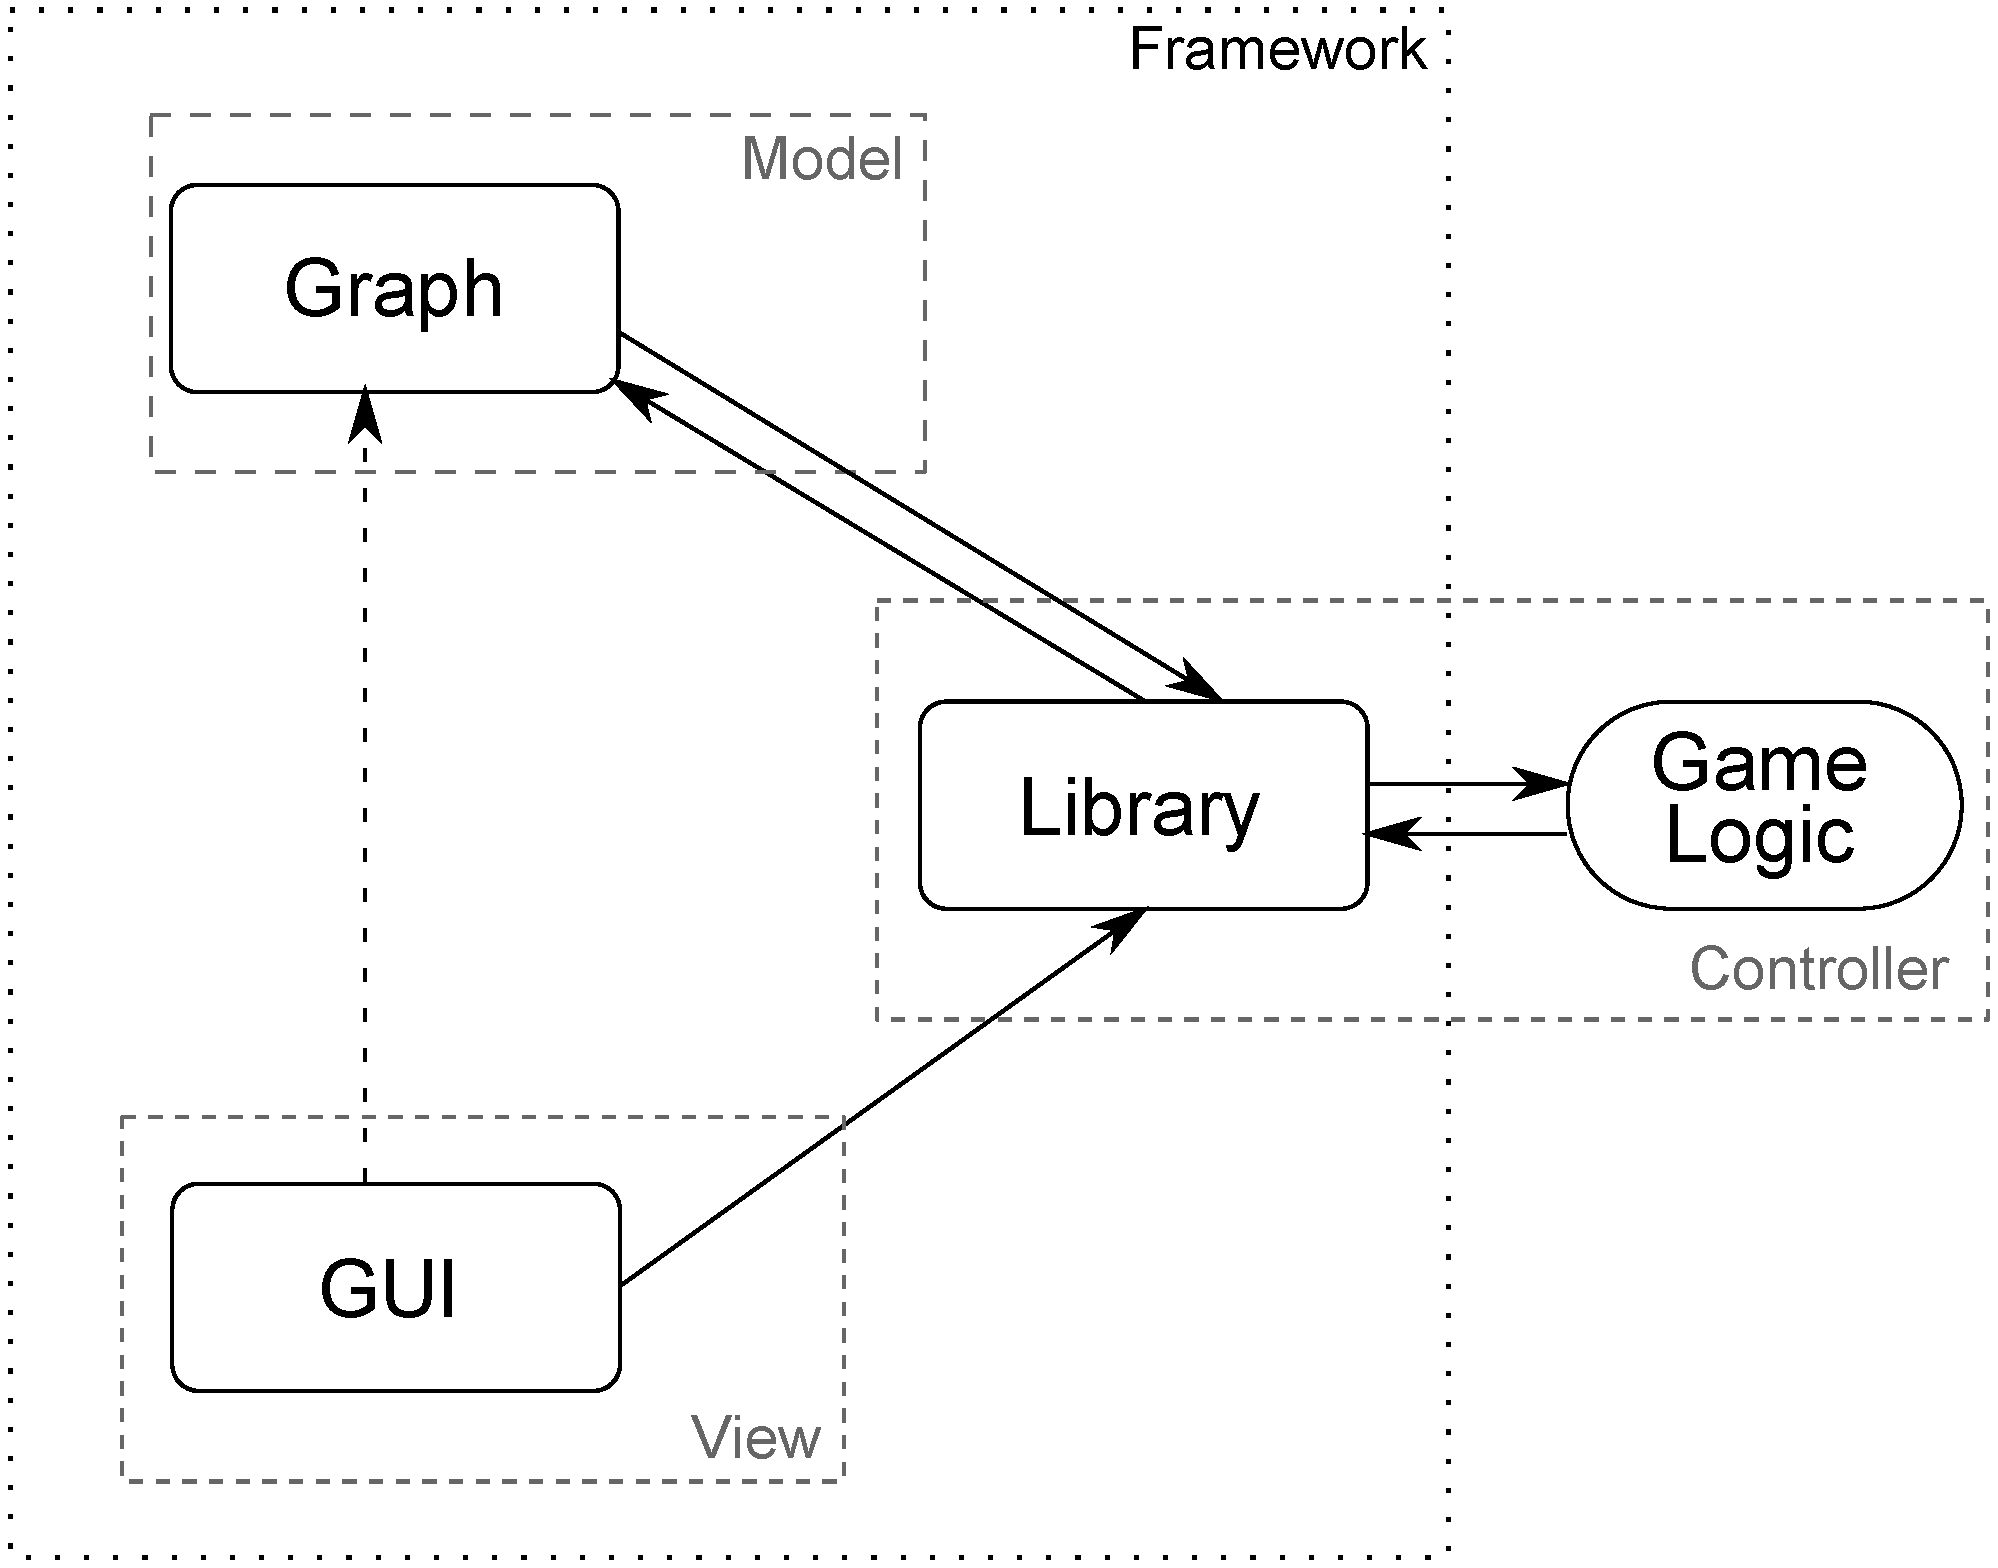
\includegraphics[width=0.8\textwidth]{mvc.pdf}
	\caption{Diagram showing the realization of the \gls{MVC} design pattern by the framework.}
	\label{img:MVC}
\end{figure}

\begin{description}
\item[Model] The model contains the structure of the \gls{game}['s] current \gls{graph}.
\item[GUI] The \gls{gui} is responsible for displaying the game, including the \gls{graph} represented by the model and the menu (see \ref{REF:GUI_GAME}). It also receives user input (e.g. mouse clicks) and passes them to the controller.
\item[Libraries] The libraries act as an interface between the game and the remaining parts of the framework. They preprocesses the user input and notify the game logic. Furthermore they are responsible for reading and modifying the \gls{graph} according to the commands of the game logic.
\item[Game Logic] The Game Logic is the component created by the \gls{developer}. It decides how the user input is handled and what modifications have to be applied to the \gls{graph}.
\end{description}